% pyInnerBubble -- main pipeline workflow (TikZ).
% Compile with: pdflatex workflow.tex   (standalone -> tight PDF of just the diagram)
\documentclass[border=12pt]{standalone}
\usepackage{tikz}
\usetikzlibrary{arrows.meta, positioning, backgrounds, fit}

% inline monospace helper used in the node labels
\newcommand{\code}[1]{{\ttfamily\scriptsize #1}}

\begin{document}
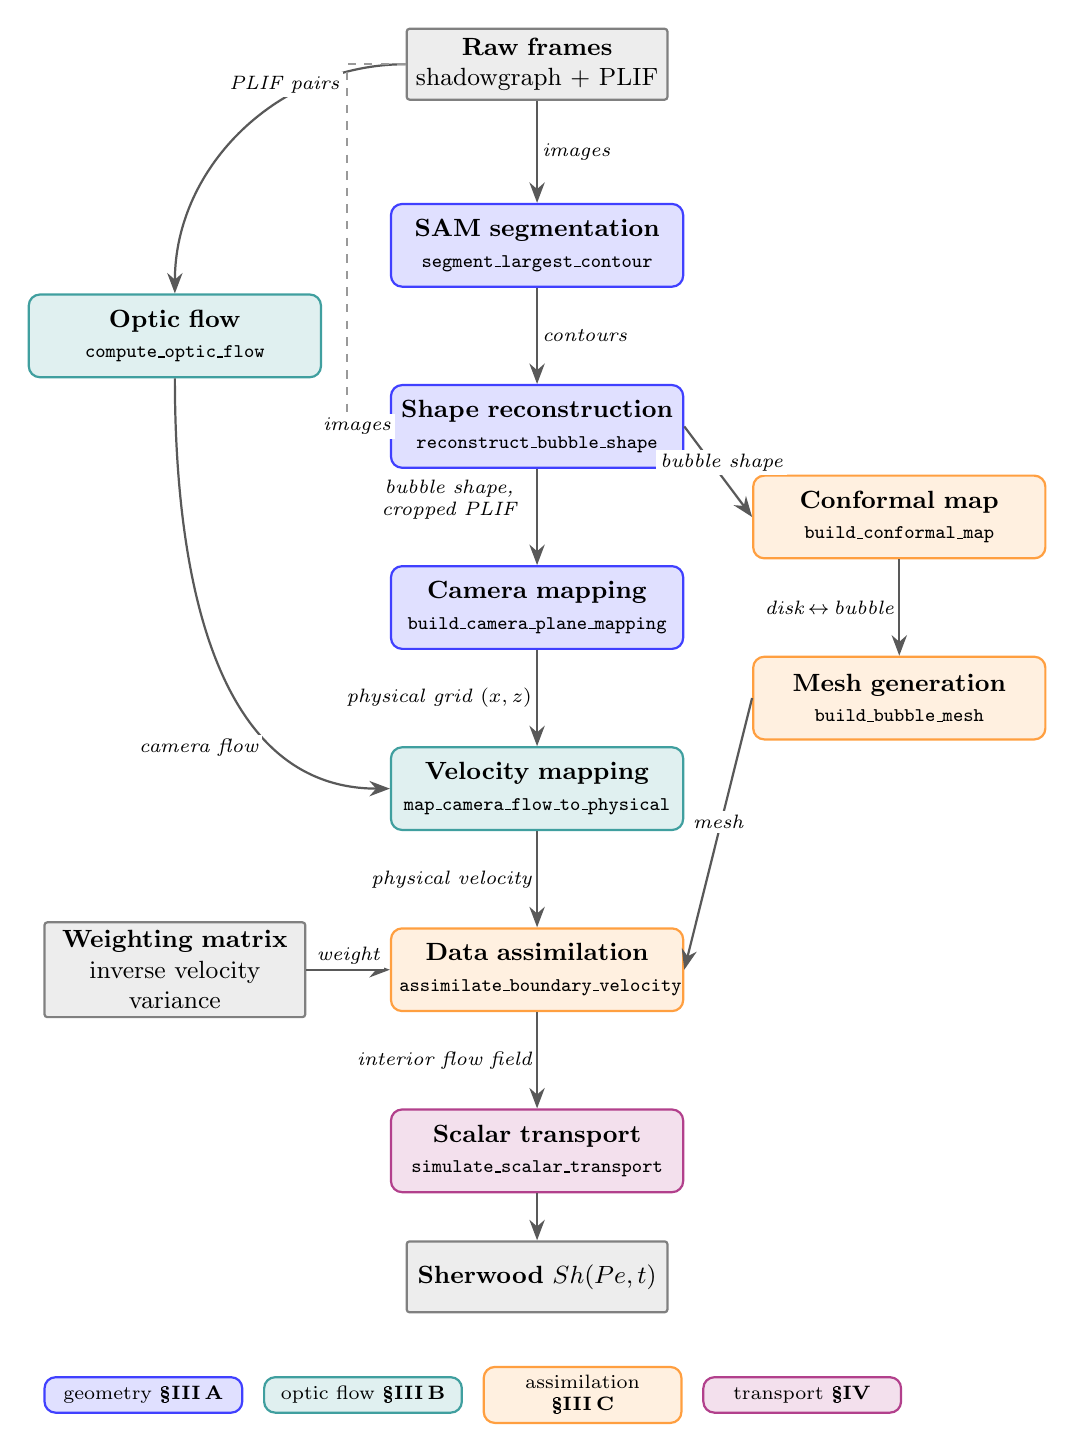
\begin{tikzpicture}[
  font=\sffamily,
  every node/.style={align=center},
  stage/.style={rounded corners=4pt, draw=#1!75, line width=0.8pt, fill=#1!12,
                text width=3.5cm, minimum height=1.05cm, inner sep=3pt, font=\small},
  io/.style={draw=black!50, line width=0.8pt, fill=black!7, rounded corners=1pt,
             text width=3.1cm, minimum height=0.9cm, inner sep=3pt, font=\small},
  a/.style={-{Stealth[length=2.6mm]}, line width=0.8pt, draw=black!65},
  a2/.style={-{Stealth[length=2.2mm]}, line width=0.7pt, draw=black!40, dashed},
  lbl/.style={font=\scriptsize\itshape, fill=white, inner sep=1.5pt, midway},
]
\colorlet{geo}{blue}
\colorlet{ofl}{teal}
\colorlet{asm}{orange}
\colorlet{trn}{violet!80!red}

% ---------- spine nodes (x = 0) ----------
\node[io]        (frames) at (0, 0)     {\textbf{Raw frames}\\ shadowgraph + PLIF};
\node[stage=geo] (sam)    at (0,-2.3)   {\textbf{SAM segmentation}\\ \code{segment\_largest\_contour}};
\node[stage=geo] (shape)  at (0,-4.6)   {\textbf{Shape reconstruction}\\ \code{reconstruct\_bubble\_shape}};
\node[stage=geo] (cammap) at (0,-6.9)   {\textbf{Camera mapping}\\ \code{build\_camera\_plane\_mapping}};
\node[stage=ofl] (velmap) at (0,-9.2)   {\textbf{Velocity mapping}\\ \code{map\_camera\_flow\_to\_physical}};
\node[stage=asm] (da)     at (0,-11.5)  {\textbf{Data assimilation}\\ \code{assimilate\_boundary\_velocity}};
\node[stage=trn] (trans)  at (0,-13.8)  {\textbf{Scalar transport}\\ \code{simulate\_scalar\_transport}};
\node[io]        (sh)     at (0,-15.4)  {\textbf{Sherwood} $Sh(Pe,t)$};

% ---------- side nodes (offset into the gaps so arrows are clean diagonals) ----------
\node[stage=ofl] (optic)  at (-4.6,-3.45) {\textbf{Optic flow}\\ \code{compute\_optic\_flow}};
\node[io]        (wt)      at (-4.6,-11.5) {\textbf{Weighting matrix}\\ inverse velocity\\ variance};
\node[stage=asm] (conf)   at ( 4.6,-5.75) {\textbf{Conformal map}\\ \code{build\_conformal\_map}};
\node[stage=asm] (mesh)   at ( 4.6,-8.05) {\textbf{Mesh generation}\\ \code{build\_bubble\_mesh}};

% ---------- spine arrows ----------
\draw[a] (frames) -- node[lbl, right]{images} (sam);
\draw[a] (sam)    -- node[lbl, right]{contours} (shape);
\draw[a] (shape)  -- node[lbl, left, pos=0.32, text width=2.1cm]{bubble shape,\\ cropped PLIF} (cammap);
\draw[a] (cammap) -- node[lbl, left]{physical grid $(x,z)$} (velmap);
\draw[a] (velmap) -- node[lbl, left]{physical velocity} (da);
\draw[a] (da)     -- node[lbl, left]{interior flow field} (trans);
\draw[a] (trans)  -- (sh);

% ---------- optic-flow branch (left) ----------
\draw[a]  (frames.west) to[out=180, in=90]  node[lbl, above, pos=0.35]{PLIF pairs} (optic.north);
\draw[a]  (optic.south) to[out=270, in=180] node[lbl, below left, pos=0.7]{camera flow} (velmap.west);
% shape reconstruction ALSO uses the raw images (secondary input) -- orthogonal, in the clear channel
\draw[a2] (frames.west) -- ++(-0.75,0) |- node[lbl, pos=0.62]{images} (shape.west);

% ---------- assimilation branch (right, staggered) ----------
\draw[a] (shape.east) -- node[lbl, above, pos=0.55]{bubble shape} (conf.west);
\draw[a] (conf) -- node[lbl, left]{disk\,$\leftrightarrow$\,bubble} (mesh);
\draw[a] (mesh.west) -- node[lbl, above, pos=0.5]{mesh} (da.east);
\draw[a] (wt) -- node[lbl, above]{weight} (da);

% ---------- legend (horizontal row at the bottom) ----------
\node[stage=geo, minimum height=0.45cm, text width=2.3cm, font=\scriptsize] (lg) at (-5.0,-16.9) {geometry \textbf{\S III\,A}};
\node[stage=ofl, right=2.5mm of lg, minimum height=0.45cm, text width=2.3cm, font=\scriptsize] (lo) {optic flow \textbf{\S III\,B}};
\node[stage=asm, right=2.5mm of lo, minimum height=0.45cm, text width=2.3cm, font=\scriptsize] (la) {assimilation \textbf{\S III\,C}};
\node[stage=trn, right=2.5mm of la, minimum height=0.45cm, text width=2.3cm, font=\scriptsize] (lt) {transport \textbf{\S IV}};

\end{tikzpicture}
\end{document}
